\documentclass[xcolor=dvipsnames]{beamer}
%\documentclass[handout,xcolor=dvipsnames]{beamer}

% == Packages for beamer
\usepackage{xcolor}
\usepackage{graphicx}
\usepackage{fancybox}
\usepackage{hyperref}
\usepackage{amsmath,amssymb,amsfonts,bm}
\usepackage{wasysym}
\usepackage{colortbl}
\usepackage{booktabs}
\usepackage[english]{babel}
\usepackage{times}
\usepackage[T1]{fontenc}
\usepackage{multirow}

% == Other Packages
\usepackage{rotating}
\usepackage{latexsym}
\usepackage{ulem}
\usepackage{tikz}
\usetikzlibrary{positioning,arrows.meta}

% == theme & colors
\usetheme{Warsaw}
\usepackage{helvet}
\definecolor{someblue}{rgb}{0,.1,0.8}
\definecolor{dgreen}{rgb}{0,.6,0.8}
\useoutertheme{infolines}

% == New Commands
\newcommand\spacingset[1]{\renewcommand{\baselinestretch}{#1}\small\normalsize}
\renewcommand\r{\right}
\renewcommand\l{\left}
\newcommand\makegaps{\addtolength{\itemsep}{.25\baselineskip}}
\newcommand\makebiggaps{\addtolength{\itemsep}{.5\baselineskip}}

% = For stats & econometrics
\renewcommand{\epsilon}{\varepsilon}
\newcommand\E{\mathbb{E}}
\newcommand\V{\mathbb{V}}
\newcommand{\Var}{\mathrm{Var}}
\newcommand{\Cov}{\mathrm{Cov}}
\newcommand\indep{\protect\mathpalette{\protect\independenT}{\perp}}
\def\independenT#1#2{\mathrel{\rlap{$#1#2$}\mkern2mu{#1#2}}}

\newtheorem{iass}{Identification Assumption}
\newtheorem{ires}{Identification Result}

\graphicspath{{figures/}{images/}}

\title[]{Selection on Observables II: Estimation}
\subtitle[ ]{PS200C, Spring 2026}
\author[Hazlett]{Chad Hazlett}
\institute[UCLA]{UCLA\\[1ex]
  \texttt{chazlett@ucla.edu}
}
\date{}

\begin{document}

\begin{frame}
  \titlepage
\end{frame}


%% =====================================================================
\section{Where we left off}
%% =====================================================================

\begin{frame}{Where we left off}
\small
\onslide<1-> \textbf{Conditional ignorability (CI):}
$$\{Y_{1i}, Y_{0i}\} \indep D_i \mid X_i$$

\medskip
\onslide<2-> Under CI (+ common support), the ATE is identified:
$$\E[Y_1 - Y_0] = \E_X\!\left[\,\E[Y \mid D=1, X] - \E[Y \mid D=0, X]\,\right]$$

\bigskip
\onslide<3-> In words: an \emph{experiment inside each stratum of $X$}, then average over $X$.

\bigskip
\onslide<4-> Understanding and arguing about CI is the hard and important thing. \\
\bigskip
\onslide<5-> Today: how to actually do the adjustment on the chosen $X$ 
\end{frame}


\begin{frame}{Roadmap}
\small
\onslide<1-> A menu of ways to turn CI into an estimate:
\begin{itemize}
\item<2-> \textbf{Subclassification} (last time)
\item<3-> \textbf{Matching} (a flexible version of subclassification)
\item<4-> \textbf{Propensity score} methods (matching, then IPW)
\item<5-> \textbf{Balancing weights} (skip the propensity score; balance directly)
\item<6-> \textbf{Regression} (via a ``regression imputation'' lens)
\end{itemize}

\bigskip
\onslide<7-> Under CI, these are all estimating the same thing.  They differ only in \textit{how they approximate conditioning on $X$}.
\end{frame}


%% =====================================================================
\section{From Subclassification to Matching}
%% =====================================================================

\begin{frame}{Recap: Subclassification}
\small
\onslide<1-> From SOO I:
\begin{itemize}
\item Partition units by $X$ into strata $x_1, x_2, \ldots$
\item Within each stratum, treated and control are exchangeable (CI).
\item Compute DIM within each stratum; weight up to the population:
$$\widehat{\tau} \;=\; \sum_x \left[\bar Y_1(x) - \bar Y_0(x)\right] \widehat{\Pr}(X = x)$$
\end{itemize}

\bigskip
\onslide<2-> Works great when $X$ is low-dimensional and discrete. \\
\bigskip
\onslide<3-> Problematic with too many variables, continuous variables: empty and under-populated strata.
\end{frame}

\begin{frame}{Matching: subclassification with 1-unit ``strata''}
\small
\begin{itemize}
\item<1-> For each treated unit $i$, find the closest control unit $j$ in $X$.
\item<2-> The pair $(i, j)$ is like a mini, approximate stratum.
\item<3-> ATT estimator:
$$\widehat{\tau}_{ATT} = \frac{1}{n_1} \sum_{i : D_i = 1} \left(Y_i - Y_{j(i)}\right)$$
\end{itemize}

\bigskip
\onslide<4-> A matched sample is just a flexible subclassification.  Same idea; the strata move with the data.
\end{frame}


\begin{frame}{What is ``closest''?}
\small
\onslide<1-> With a single $X$: obvious --- smallest $|X_i - X_j|$.

\medskip
\onslide<2-> With several $X$: need a distance metric.
\begin{itemize}
\item \textbf{Euclidean}: $\|X_i - X_j\|$ --- scale-sensitive.
\item \textbf{Mahalanobis}: $\sqrt{(X_i - X_j)' \widehat{\Sigma}_X^{-1} (X_i - X_j)}$ --- scale-invariant, accounts for correlation.
\end{itemize}

\bigskip
\onslide<3->
\begin{center}
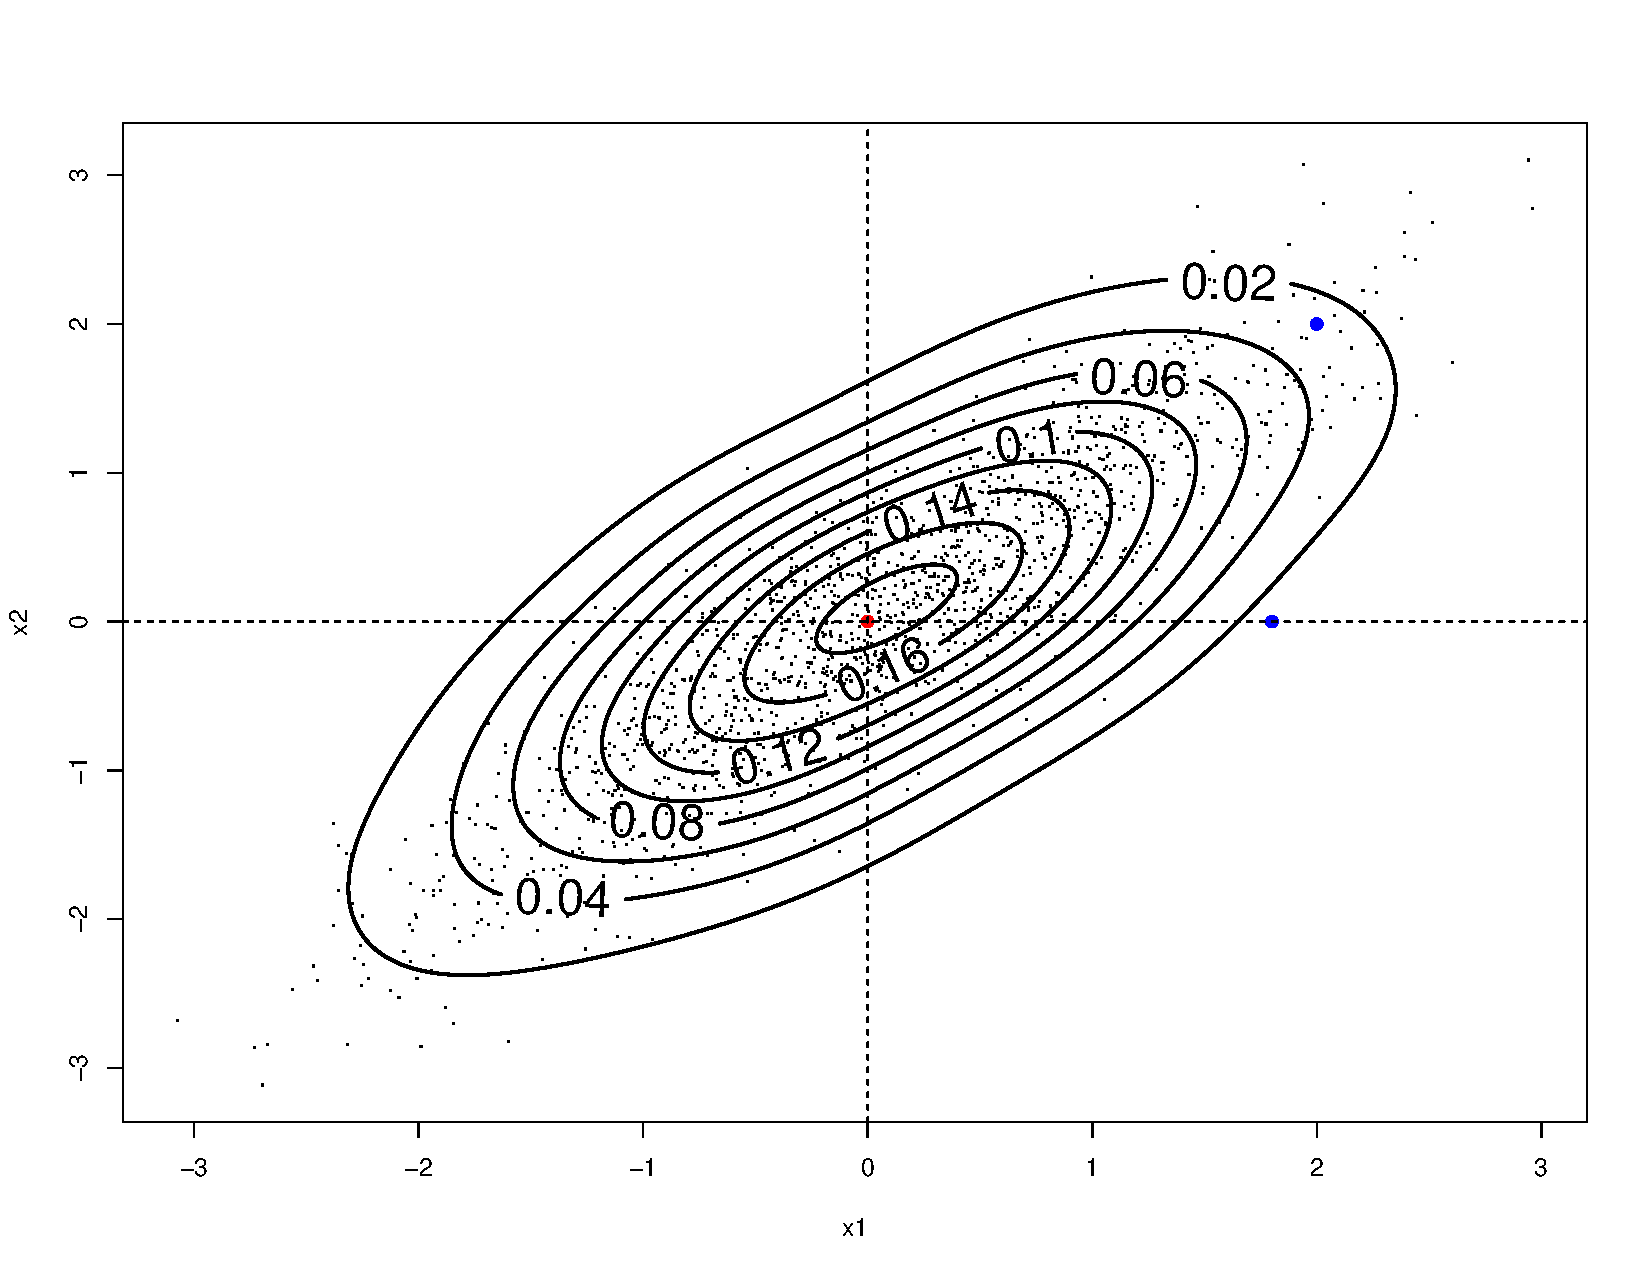
\includegraphics[width=0.45\textwidth]{Maha1.pdf}
\end{center}
\end{frame}

\begin{frame}{The limits of matching}
\small
\onslide<1-> Problem: unlike true stratification, the treated and control getting compared aren't exactly the same on $X_i$.
\begin{itemize}
\footnotesize
\item There is a \textit{discrepancy}, $\|X_i-X_j\|$, between treated and control units in a pair $\rightarrow$ difference in $Y_i(1)$ and $Y_j(0)$.  This bias does not vanish at the usual $\sqrt n$ rate (Abadie \& Imbens, 2006).
\item As $\dim(X)$ grows, the distance to even your nearest neighbor rapidly increases (``curse-of-dimensionality'').
\end{itemize}

\bigskip
\small
\onslide<2-> One solution: \textbf{bias adjustment} (Abadie \& Imbens, 2011).
\begin{itemize}
\footnotesize
\item Regress $Y \sim X$ among controls; call the fit $\widehat{\mu}_0(X)$.
\item Use $\widehat{\mu}_0(X_i) - \widehat{\mu}_0(X_{j(i)})$ to estimate the $Y(0)$ gap implied by the $X$-discrepancy, and subtract it from each matched pair.
\end{itemize}
\end{frame}


%% =====================================================================
\section{Propensity Score: a dimension reducer}
%% =====================================================================

\begin{frame}{The propensity score}
\small
\onslide<1-> Another solution: Find just one dimension that really counts. \\
\medskip
\onslide<2-> The propensity score is the probability of treatment given $X$:\\

$$\pi(X) \;=\; \Pr(D = 1 \mid X)$$

\medskip
\onslide<3-> \textbf{Rosenbaum \& Rubin (1983)}: if CI holds given $X$, it also holds given $\pi(X)$.\\
$$\{Y_1, Y_0\} \indep D \mid X \quad \Longrightarrow \quad \{Y_1, Y_0\} \indep D \mid \pi(X)$$

\bigskip
\onslide<4-> Instead of matching in high-dimensional $X$, just a scalar!
\end{frame}


\begin{frame}{Propensity score matching, on Blattman \& Annan example}
\small
\onslide<1-> Recipe:
\footnotesize
\begin{enumerate}
\item Fit $\widehat{\pi}(X)$ (e.g., logistic regression of $D$ on $X$).
\item For each treated $i$, find the control $j$ with the closest $\widehat{\pi}(X_j)$.
\item Compute DIM on the matched sample.
\end{enumerate}
\vspace{-.5cm}
\small
\begin{columns}[T]
\begin{column}{0.5\textwidth}
\onslide<2->
\begin{center}
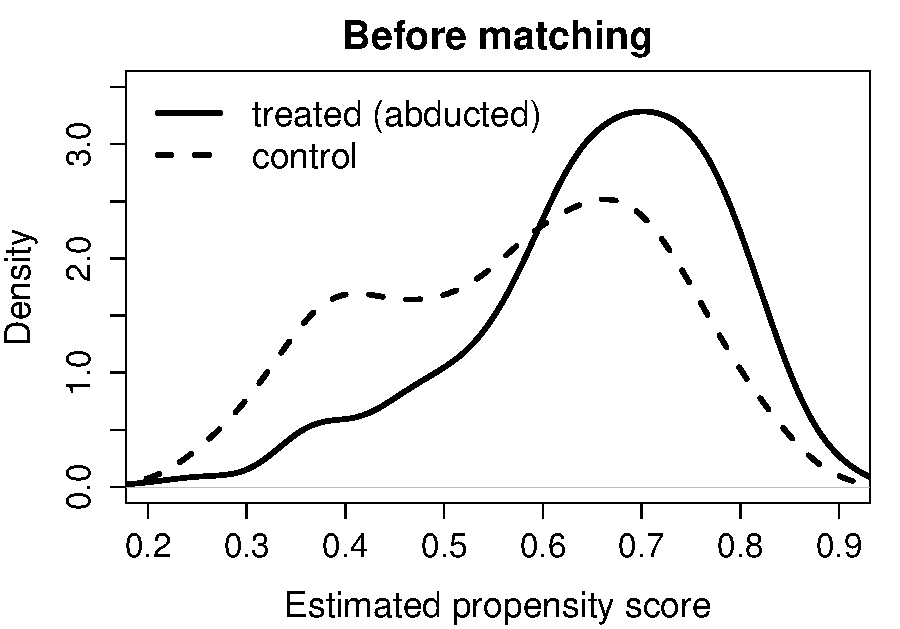
\includegraphics[width=.9\textwidth]{blattman_pscore_pre.pdf}
\end{center}
\end{column}
\begin{column}{0.5\textwidth}
\onslide<3->
\begin{center}
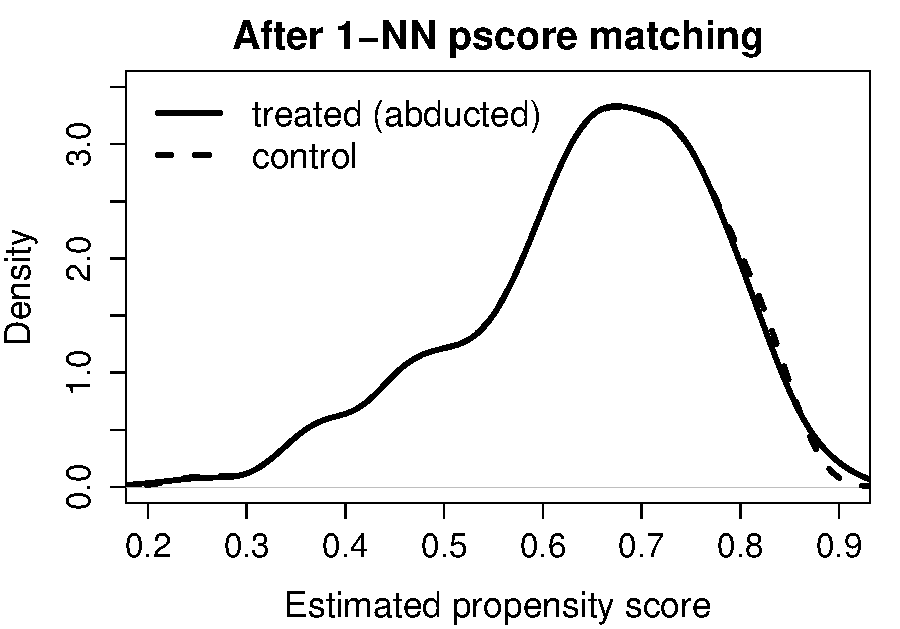
\includegraphics[width=.9\textwidth]{blattman_pscore_post.pdf}
\end{center}
\end{column}
\end{columns}

\vspace{2pt}
\onslide<4-> \footnotesize Caveats: Extreme $\pi$ may need to be trimmed; depends on how well we estimate $\pi(X)$ 
\end{frame}


%% =====================================================================
\section{Inverse Propensity Weighting (IPW)}
%% =====================================================================

\begin{frame}{From matching to weighting}
\small
\onslide<1-> Is there a better way to use the pscore without the wasted sample and discrepancy from matching?

\medskip
\onslide<2-> Intuition: rare treated units (low $\pi$) represent many similar untreated units.  So count them more.

\bigskip
\onslide<3-> \textbf{IPW weights:}
$$w_i \;=\; \frac{D_i}{\widehat{\pi}(X_i)} \;+\; \frac{1 - D_i}{1 - \widehat{\pi}(X_i)}$$

\bigskip
\onslide<4-> Treated units with low $\pi$: upweighted (they're rare).\\
Control units with high $\pi$: upweighted (also rare).
\end{frame}


\begin{frame}{Weights: What we want vs what we have}
\footnotesize
\onslide<1-> Under CI, the ATE is an average of within-$X$ effects over the \emph{overall} $X$-distribution:\\
$$\E[\tau] = \int \underbrace{\left\{\E[Y \mid D=1, X] - \E[Y \mid D=0, X]\right\}}_{\text{within-}X\text{ effect}} \;\textcolor{red}{p(X)}\; dx$$

\medskip
\onslide<2-> But the raw DIM averages each arm over the \emph{wrong} distribution:\\
$$\text{DIM} = \int \E[Y\mid D{=}1, X]\,\textcolor{orange}{p(X\mid D{=}1)}\, dx \;-\; \int \E[Y\mid D{=}0, X]\,\textcolor{dgreen}{p(X\mid D{=}0)}\, dx$$

\bigskip
\onslide<3-> Treated units live in $\textcolor{orange}{p(X\mid D{=}1)}$; controls in $\textcolor{dgreen}{p(X\mid D{=}0)}$.  We want both to live in $\textcolor{red}{p(X)}$.

\bigskip
\onslide<4-> Weights can do this...
\end{frame}


\begin{frame}{The weights that close the gap}
\small
\onslide<1-> To turn $\textcolor{orange}{p(X\mid D{=}1)}$ into $\textcolor{red}{p(X)}$, multiply by $\dfrac{\textcolor{red}{p(X)}}{\textcolor{orange}{p(X\mid D{=}1)}}$.  Same idea for controls.

\medskip
\onslide<2-> In either arm, such a weight has the form:
$$w_i \;=\; \frac{p(X_i)}{p(X_i \mid D_i)}$$

\bigskip
\onslide<3-> By Bayes' rule:
$$\frac{p(X_i)}{p(X_i \mid D_i)} \;=\; \frac{p(D_i)}{p(D_i \mid X_i)}$$

\bigskip
\onslide<4-> So the weight for each unit is $\dfrac{p(D_i)}{p(D_i \mid X_i)}$ --- the \textbf{stabilized IPW weights}:
\footnotesize
$$w_i^{\text{stab}} \;=\; \frac{D_i\, \Pr(D{=}1)}{\widehat{\pi}(X_i)} \;+\; \frac{(1-D_i)\, \Pr(D{=}0)}{1 - \widehat{\pi}(X_i)}$$

\bigskip
\footnotesize
\onslide<5-> Drop the $p(D_i)$ in numerator and you'd have the plain IPW above ($1/\widehat{\pi}(X_i)$ or $1/(1-\widehat{\pi}(X_i))$), which has higher variance.
\end{frame}


\begin{frame}{IPW in pictures}
\small
\onslide<1-> Before weighting, treated and control differ in $X$:
\begin{center}
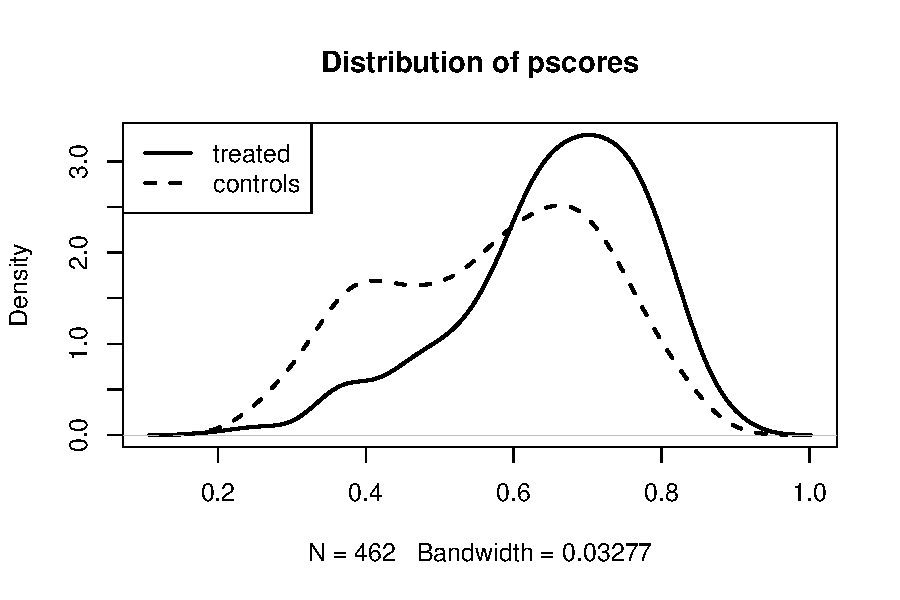
\includegraphics[width=0.42\textwidth]{pscores_pre.pdf}
\end{center}

\onslide<2-> After IPW, the control distribution is reshaped to match the treated:
\begin{center}
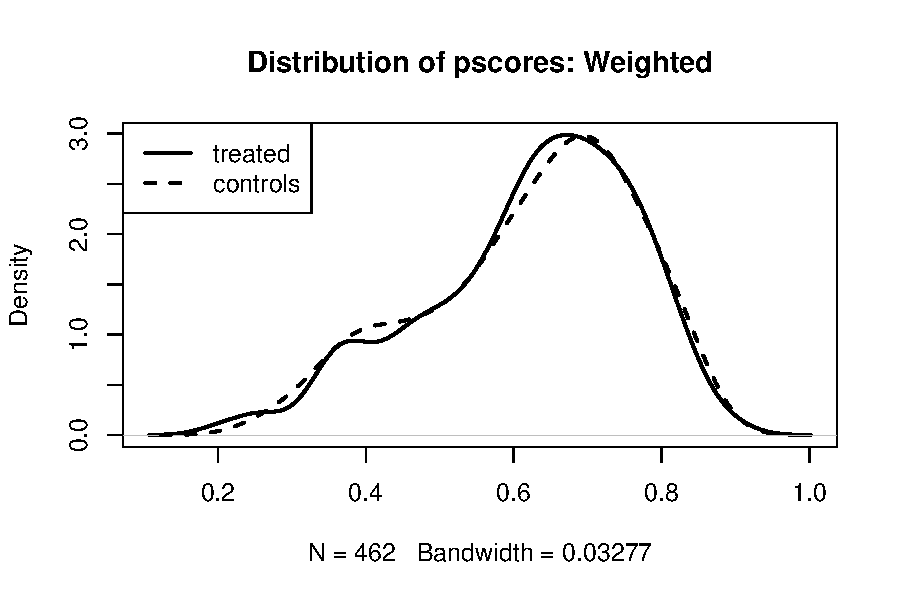
\includegraphics[width=0.42\textwidth]{pscores_post.pdf}
\end{center}
\end{frame}


\begin{frame}{IPW caveats}
\small
\onslide<1-> What can go wrong:
\bigskip

\small
\begin{itemize}
\item<1-> \textbf{Extreme weights/ poor overlap}:  $\widehat{\pi}(X) \approx 0$ or $1$ $\Rightarrow$ enormous weights $\Rightarrow$ huge variance, signal of non-overlap (extrapolation)
\bigskip
\item<2-> \textbf{Misspecification.}  $\widehat{\pi}(X)$ wrong $\Rightarrow$ weights wrong $\Rightarrow$ bias.
\bigskip
\item<3-> Trimming is sometimes used to address extreme weights...changes the estimate, can be arbitrary. 
\end{itemize}
\end{frame}


%% =====================================================================
\section{Balancing Weights}
%% =====================================================================

\begin{frame}{Wait --- why estimate $\pi(X)$ at all?}
\small
\onslide<1-> If you really just want get treated and control onto the same distribution in $X$, why not just weight to make it so?\\ 
\bigskip
\onslide<2-> Choose weights $w_i$ to satisfy, e.g., \textbf{mean balance on $X$}:
$$\sum_{i: D_i = 1} w_i X_i \;=\; \sum_{i: D_i = 0} w_i X_i$$

\medskip
\onslide<2-> ...subject to a regularizer (keep weights as close to uniform as possible).

\bigskip
\onslide<3-> E.g. maximum entropy balancing (Hainmueller, 2012) minimizes $\sum_i w_i log(w_i)$ while achieving the target balance conditions. 
\end{frame}

\begin{frame}{Balance on Blattman \& Annan}
\begin{center}
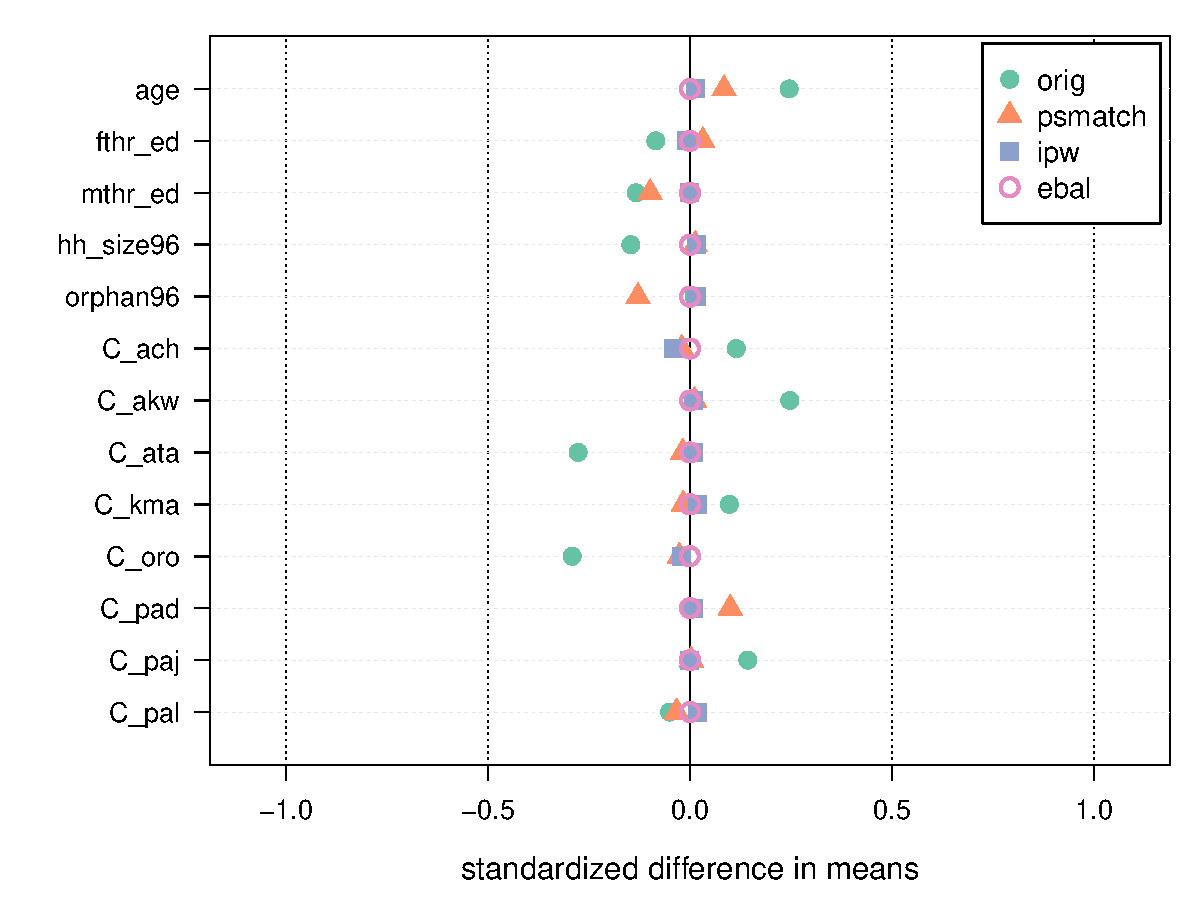
\includegraphics[width=0.75\textwidth]{all_blattman.pdf}
\end{center}
\vspace{-.2cm}
\footnotesize Standardized mean differences, 13 covariates.  ``orig'' = no adjustment.
\end{frame}

\begin{frame}{How much balance?}
\small
\onslide<1-> Mean balance on $X$ is not full distributional balance.

\medskip
\onslide<2-> You can ask for more:
\begin{itemize}
\item higher moments of $X$,
\item interactions,
\item kernels / non-parametric balance (e.g. kernel balancing).
\end{itemize}

\bigskip
\onslide<3-> Tradeoff: you only ensure balance on the things you target, but you get perfect balance on them in the sample, don't need correct pscore. %A modeling choice, \emph{transparent}: you stipulate what balance you want and achieve it exactly.  Contrast with IPW, where balance is a hoped-for byproduct of a correct $\pi(X)$.
\end{frame}


%% =====================================================================
\section{Regression, via imputation}
%% =====================================================================

\begin{frame}{Regression --- start with imputation}
\small
\onslide<1-> What's actually missing?  For each unit $i$ with covariates $X_i$:
\begin{itemize}
\item If $D_i = 1$, we observe $Y_i(1)$; we don't know $Y_i(0)$.
\item If $D_i = 0$, we observe $Y_i(0)$; we don't know $Y_i(1)$.
\end{itemize}

\bigskip
\onslide<2-> \textbf{Idea}: \emph{impute} the missing potential outcome using $\mu_d(x) \equiv \E[Y(d) \mid X = x]$:
\begin{itemize}
\item Fit $\widehat{\mu}_1(x)$ on treated units (estimates $\E[Y(1) \mid X{=}x]$).
\item Fit $\widehat{\mu}_0(x)$ on control units (estimates $\E[Y(0) \mid X{=}x]$).
\item For each $i$, predict both: $\widehat{Y}_i(1) = \widehat{\mu}_1(X_i)$, $\widehat{Y}_i(0) = \widehat{\mu}_0(X_i)$.
\end{itemize}

\bigskip
\onslide<3-> Average the individual-level differences:
$$\widehat{\tau} = \frac{1}{n}\sum_i \left[\widehat{\mu}_1(X_i) - \widehat{\mu}_0(X_i)\right]$$

\medskip
\onslide<4-> This is \textbf{regression imputation}, a.k.a.\ \textbf{$g$-computation}.  As natural a use of regression as there is.
\end{frame}


\begin{frame}{Linear models $\Rightarrow$ Lin's estimator}
\small
\onslide<1-> Suppose $\widehat{\mu}_1$ and $\widehat{\mu}_0$ are linear:
$$\widehat{\mu}_d(x) = \widehat{\alpha}_d + \widehat{\beta}_d' x, \quad d \in \{0, 1\}$$

\bigskip
\onslide<2-> Fitting \emph{separate} linear models on treated and control and then averaging predicted differences is exactly the interacted OLS regression
$$Y = \alpha + \tau D + \beta' X + \gamma'(X \cdot D) + \varepsilon$$
evaluated at the overall mean of $X$.

\bigskip
\onslide<3-> This is \textbf{Lin's (2013) estimator} --- which you already saw in experiments.  The same thing, just now motivated by ``impute each unit's missing PO.''
\end{frame}


\begin{frame}{What about pooled OLS?}
\small
\onslide<1-> The usual regression $Y = \alpha + \tau D + \beta' X + \varepsilon$ (no interaction):
\begin{itemize}
\footnotesize
\item<2-> Assumes the same slope in $X$ for treated and control.
\item<3-> Equivalent to fitting a \emph{pooled} $\widehat{\mu}(x)$ and taking $\widehat{\tau}$ from the $D$ coefficient.
\item<4-> When treatment effects vary with $X$: $\widehat{\tau}$ is a weighted average of unit-level effects, with weights that tilt toward units in the region of overlap --- not necessarily the ATE or ATT.
\end{itemize}
\small
\bigskip
\onslide<5-> Fix: either use the interacted (Lin) version, or commit to the assumption that slopes are equal.
\end{frame}


%% =====================================================================
\section{All roads lead to the same place}
%% =====================================================================

\begin{frame}{All roads lead to the same place}
\small
\onslide<1-> Under CI, every method on the menu is trying to estimate
$$\E_{X \sim F}\!\left[\,\mu_1(X) - \mu_0(X)\,\right]$$
\footnotesize
\begin{itemize}
\item $F$ is a choice of estimand: $F = p(X)$ gives the ATE; $p(X \mid D{=}1)$ gives the ATT; $p(X \mid D{=}0)$ gives the ATC.
\item the ``adjusting for $X$'' is borne out by using the same $F$ for both treated and controls
\end{itemize}
\medskip
\small
\medskip
\onslide<3-> They achieve this by different strategies:
\medskip

\begin{center}
{\footnotesize
\begin{tabular}{ll}
\toprule
\textbf{Method} & \textbf{How it conditions on $X$} \\
\midrule
Subclassification & coarse strata of $X$ \\
Matching & nearest-neighbor ``strata'' in $X$ \\
Pscore matching & match on $\widehat{\pi}(X)$ \\
IPW & reweight by $1/\widehat{\pi}(X)$ \\
Balancing weights & solve for weights balancing $X$ \\
Regression imputation & model $\mu_d(X)$ and impute \\
\bottomrule
\end{tabular}
}
\end{center}
\end{frame}


\begin{frame}{Blattman \& Annan: ATT across methods}
\small
\begin{center}
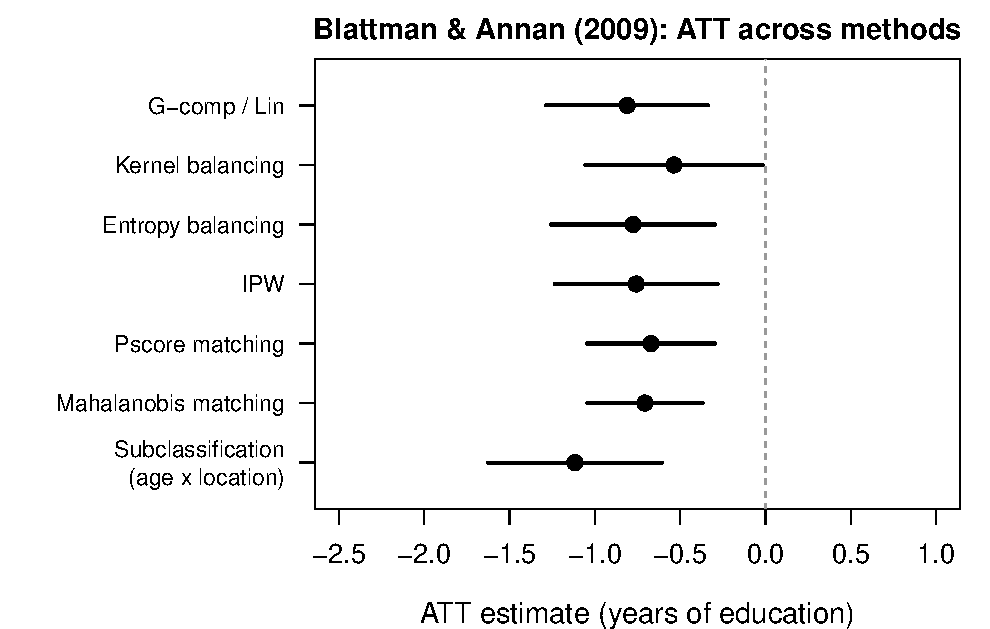
\includegraphics[width=0.72\textwidth]{blattman_estimates.pdf}
\end{center}
\vspace{-.2cm}
{\tiny Covariates: age, fthr\_ed, mthr\_ed, hh\_size96, orphan96, and 8 location dummies.}

\smallskip

\small If everything agrees, great; if not, diagnose.

\end{frame}


\begin{frame}{Beyond: combining pscore and outcome model}
\small
\onslide<1-> So far: estimate either $\widehat{\pi}(X)$ (weighting) \emph{or} $\widehat{\mu}_d(X)$ (regression).

\bigskip
\onslide<2-> \textbf{Doubly robust} methods combine both:
\begin{itemize}
\footnotesize
\item \textbf{AIPW}: IPW estimator + regression adjustment using $\widehat{\mu}_d(X)$.
\item \textbf{TMLE}: iteratively update $\widehat{\mu}_d$ using $\widehat{\pi}$.
\item \textbf{Double ML (DML)}: plug flexible (ML-based) $\widehat{\pi}$ and $\widehat{\mu}_d$ into AIPW with cross-fitting.
\end{itemize}
\onslide<3-> Consistent if \textit{either} $\widehat{\pi}$ or $\widehat{\mu}_d$ is correctly specified.  Good inference with flexible (ML) fits if both converge fast enough.

%\bigskip
%\onslide<4-> \textbf{Why not just crank up flexibility in g-comp alone?}  Overfit $\widehat{\mu}_d$ can extrapolate wildly where overlap is weak; with DR, the weighting piece keeps you honest in the overlap region.

\bigskip
\onslide<5-> All still need CI + common support.  Flexibility buys you less bias from model form, not from missing confounders.
\end{frame}


%\begin{frame}{Which should you use?}
%\small
%\onslide<1-> There is no ``best.''  Consider:
%\begin{itemize}
%\item<1-> \textbf{Transparency.}  Can you explain what the estimator is doing, and show it worked (balance, overlap)?
%\item<2-> \textbf{Robustness.}  Is your answer sensitive to modeling choices ($\pi$-score form, which $X$, interactions)?
%\item<3-> \textbf{Interpretability.}  Matched samples are easy to describe; regression coefficients less so when effects are heterogeneous.
%\item<4-> \textbf{Efficiency.}  Weighting and regression keep all units; matching often discards.
%\end{itemize}
%
%\bigskip
%\onslide<5-> \textbf{Reasonable practice}: In a given setting, take whatever approaches are most appropriate and show them all. 
%\end{frame}


%% =====================================================================
\section{Wrap}
%% =====================================================================

\begin{frame}{Takeaways}
\small
\begin{itemize}
\item<1-> \textbf{CI does the identifying work.}  Estimation is a menu of ways to operationalize ``experiment within strata of $X$.''
\medskip
\item<2-> \textbf{Subclassification} breaks in high-$d$; \textbf{matching} is the flexible version; the \textbf{propensity score} is a dimension reducer.
\medskip
\item<3-> \textbf{IPW} reweights rather than matches; \textbf{balancing weights} skip the $\pi(X)$ step and enforce balance directly.
\medskip
\item<4-> \textbf{Regression} is natural when framed as imputation: model $\mu_d(X)$, predict each unit's missing PO (or both), average over intended group.
\medskip
\item<5-> \textbf{Reasonable practice}: In a given setting, you might take one estimator as central, but good to show range of answers you get under whichever approaches are appropriate. 
\end{itemize}
\end{frame}


\end{document}
